\documentclass[border=5mm]{standalone}
\usepackage{pgfplots}
\usetikzlibrary{arrows.meta}
\pgfplotsset{compat=1.18}
\usepgfplotslibrary{fillbetween}
\begin{document}
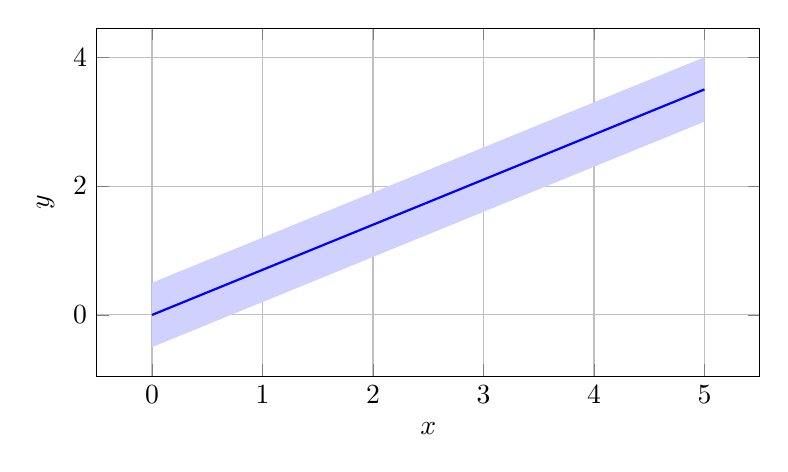
\begin{tikzpicture}[>=Stealth]
\begin{axis}[width=10cm,height=6cm,grid=major,xlabel={$x$},ylabel={$y$}]

\addplot[name path=upper,draw=none,domain=0:5]{.7*x+.5};
\addplot[name path=lower,draw=none,domain=0:5]{.7*x-.5};
\addplot[blue!18]fill between[of=upper and lower];
\addplot[blue,thick,domain=0:5]{.7*x};
\end{axis}
\end{tikzpicture}
\end{document}
